\documentclass[12pt,a4paper,oneside]{report}
\usepackage[T1]{fontenc}
\usepackage[utf8]{inputenc}
\usepackage[french]{babel}
\usepackage{lmodern}
\usepackage[margin=2.5cm,headheight=32pt]{geometry}
\usepackage{amsmath,amssymb}
\usepackage{graphicx}
\usepackage{array,booktabs,longtable}
\usepackage{xcolor}
\usepackage{tikz}
\usepackage{pgfornament}
\usepackage[skins,breakable]{tcolorbox}
\usetikzlibrary{calc,shadows}
\usepackage{titlesec}
\usepackage{etoc}
\usepackage{fancyhdr}
\usepackage{hyperref}

\definecolor{bleufonce}{HTML}{102F54}
\definecolor{bleuclair}{HTML}{EFF3F8}

\newtcolorbox{introductionchapitre}{
  enhanced,
  breakable,
  colback=bleuclair,
  colframe=bleufonce!35,
  boxrule=0.5pt,
  borderline west={2pt}{0pt}{bleufonce},
  arc=2mm,
  left=4mm,right=4mm,top=3mm,bottom=3mm,
  before skip=0pt,after skip=12pt,
  before upper={\setlength{\parindent}{0pt}}
}

\hypersetup{
  colorlinks=true,
  linkcolor=bleufonce,
  citecolor=bleufonce,
  urlcolor=bleufonce,
  pdftitle={Estimation du service de capital au Sénégal},
  pdfauthor={Anta NDAO}
}

\newcommand{\theme}{Estimation du service de capital au Sénégal}
\newcommand{\anneeacademique}{Décembre 2026}
\newcommand{\structureaccueil}{Structure d'accueil : à compléter}

\setlength{\parindent}{1.25em}
\setlength{\parskip}{0.4\baselineskip}
\renewcommand{\baselinestretch}{1.15}
\setcounter{secnumdepth}{2}
\setcounter{tocdepth}{2}

\pagestyle{fancy}
\fancyhf{}
\fancyhead[L]{\parbox[b]{\headwidth}{%
  \small\color{bleufonce}\raggedright\nouppercase{\leftmark}}}
\fancyfoot[C]{\color{bleufonce}\thepage}
\renewcommand{\headrulewidth}{0.4pt}
\renewcommand{\chaptermark}[1]{\markboth{Chapitre \thechapter~: #1}{}}
\fancypagestyle{plain}{
  \fancyhf{}
  \fancyfoot[C]{\color{bleufonce}\thepage}
  \renewcommand{\headrulewidth}{0pt}
}

\titleformat{\chapter}[display]
  {\fontsize{18}{22}\selectfont\bfseries\color{bleufonce}}
  {\filleft
    \begin{tikzpicture}
      \node[fill=bleufonce,text=white,minimum width=2.8cm,
        minimum height=2.8cm,inner sep=0pt,
        font=\normalfont\fontsize{44}{48}\selectfont]
        (numerochapitre) {\thechapter};
      \node[rotate=90,anchor=south,text=bleufonce,inner sep=0pt,
        font=\normalfont\fontsize{16}{19}\selectfont]
        at ([xshift=-0.15cm]numerochapitre.west) {CHAPITRE};
    \end{tikzpicture}}
  {12pt}{\raggedleft\MakeUppercase}
\titleformat{name=\chapter,numberless}[block]
  {\fontsize{18}{22}\selectfont\bfseries\color{bleufonce}}{}{0pt}{\raggedright\MakeUppercase}
  [{\vspace{0.3cm}\color{bleufonce}\titlerule[0.8pt]}]
\titlespacing*{\chapter}{0pt}{0pt}{24pt}
\titleformat{\section}
  {\Large\bfseries\color{bleufonce}\raggedright}
  {\colorbox{bleufonce}{\color{white}\thesection}}{0.7em}{}
  [\color{bleufonce}\titlerule]
\titlespacing*{\section}{0pt}{24pt}{14pt}
\titleformat{\subsection}
  {\large\bfseries\color{bleufonce}}{\thesubsection}{0.7em}{}

\newcommand{\rubrique}[1]{%
  \chapter*{#1}
  \phantomsection
  \addcontentsline{toc}{chapter}{#1}
  \markboth{#1}{}
}

\addto\captionsfrench{%
  \renewcommand{\listfigurename}{Liste des graphiques}
  \renewcommand{\figurename}{Graphique}
  \renewcommand{\tablename}{Tableau}
}

\begin{document}

\begin{titlepage}
\newgeometry{left=2cm,right=2cm,top=2cm,bottom=2cm}
\begin{tikzpicture}[remember picture,overlay]
  \draw[bleufonce,line width=8mm]
    (current page.south west) rectangle (current page.north east);
\end{tikzpicture}
\centering
\setlength{\parskip}{0pt}
\newcommand{\separateurcouverture}{%
  \begin{tikzpicture}
    \draw[bleufonce,line width=0.4pt] (-8,0)--(8,0);
    \node[fill=white,inner sep=0pt] {\pgfornament[width=11.5cm,color=bleufonce]{88}};
  \end{tikzpicture}\par
}
{République du Sénégal\par}
\vspace{0.4cm}

\includegraphics[height=2cm]{assets/armoiries-senegal.png}\par
\vspace{0.35cm}
{Ministère de l'Économie, des Finances et du Plan\par}
\vspace{0.25cm}

\includegraphics[width=4.5cm]{assets/logo-ministere.jpg}\par
\vspace{0.35cm}
{Agence nationale de la Statistique et de la Démographie\par}
\vspace{0.35cm}
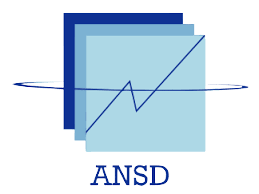
\includegraphics[height=1.6cm]{assets/logo-ansd-isecl.png}\par
\vspace{0.5cm}
{École nationale de la Statistique et de l'Analyse économique Pierre NDIAYE\par}
\vspace{0.3cm}

\includegraphics[height=1.4cm]{assets/logo-ensae-isecl.png}\par
\vspace{0.8cm}
\begin{tikzpicture}
  \node[fill=bleufonce,text=white,rounded corners=3pt,
    inner xsep=0.2cm,inner ysep=0.12cm] {\small\bfseries RAPPORT DE STAGE};
\end{tikzpicture}\par
\vspace{0.35cm}
\separateurcouverture
\vspace{0.35cm}
{\large\bfseries\color{bleufonce}\MakeUppercase{\theme}\par}
\vspace{0.35cm}
\separateurcouverture
\vspace{0.45cm}
\begingroup
\fontsize{14}{17}\selectfont
{\color{bleufonce}Rédigé par :\par}
\vspace{0.4cm}
{\bfseries Anta NDAO\par}
\vspace{0.25cm}
{\itshape Élève ingénieure statisticienne économiste en troisième année\par}
\vspace{0.55cm}
{\color{bleufonce}Maître de stage :\par}
\vspace{0.35cm}
{\bfseries M. Abdou TINE\par}
\vspace{0.25cm}
{\itshape Ingénieur Statisticien Économiste\par}
\vfill
\begin{tikzpicture}
  \node[draw=bleufonce,fill=bleuclair,text=bleufonce,
    line width=0.8pt,rounded corners=3pt,
    inner xsep=0.7cm,inner ysep=0.3cm]
    {\bfseries\anneeacademique};
\end{tikzpicture}\par
\endgroup
\end{titlepage}
\restoregeometry

\pagenumbering{roman}
\rubrique{Décharge}

\rubrique{Remerciements}

\rubrique{Dédicaces}

\rubrique{Avant-propos}

Créée en 2008, l'École nationale de la Statistique et de l'Analyse économique Pierre
Ndiaye (ENSAE) est une institution à vocation régionale, à l’image des autres écoles du Réseau
des Écoles de Statistiques africaines (RESA). Depuis la rénovation pédagogique de 2020,
l’offre de formation via concours s’y décline en deux filières~: Analyste statisticien (AS) et
Ingénieur statisticien économiste (ISE). Cette dernière filière, de niveau master, s’étend sur trois
ans (cycle court) pour les étudiants entrant avec un diplôme de licence ou après deux années en
classes préparatoires scientifiques. Elle peut également être suivie sur cinq ans (cycle long)
pour ceux entrant directement après le baccalauréat.

Les ISE développent la capacité à étudier et résoudre des problèmes complexes en mobilisant
des connaissances scientifiques, notamment en mathématiques, statistiques, économie et
finance. Ils acquièrent également des compétences en gestion d'équipe, leadership, management
de projets et ouverture culturelle, afin de s'intégrer dans des organisations et de les faire
évoluer.

À la fin de la deuxième année du cycle long, les élèves ISE effectuent un stage d’immersion de
deux mois. Ce stage leur permet de mettre en pratique les connaissances acquises et de se
familiariser avec les outils statistiques, en même temps qu’ils découvrent les réalités du monde
professionnel.

Le présent rapport s’inscrit dans ce cadre. Il sanctionne la fin d’un stage réalisé à la Division de
la Comptabilité nationale (DCN) du 12 août au 02 octobre 2026 et sera soutenu devant un
jury. Le thème de l’étude est~: \textbf{\theme}.

\rubrique{Sommaire}
\begingroup
\renewcommand{\baselinestretch}{1}
\small
\setlength{\parskip}{0pt}
\etocsetnexttocdepth{chapter}
\etocsettocstyle{}{}
\tableofcontents
\endgroup

\rubrique{Liste des sigles et acronymes}

\clearpage
\phantomsection
\addcontentsline{toc}{chapter}{Liste des graphiques}
\listoffigures
\markboth{Liste des graphiques}{}

\clearpage
\phantomsection
\addcontentsline{toc}{chapter}{Liste des tableaux}
\listoftables
\markboth{Liste des tableaux}{}

\rubrique{Résumé}

\rubrique{Abstract}

\clearpage
\pagenumbering{arabic}
\rubrique{Introduction}
\begingroup
\setlength{\parskip}{0.15\baselineskip}

L’accumulation du capital est l’un des principaux déterminants de la croissance économique sénégalaise. En
effet, la formation brute de capital fixe (FBCF) s’est accrue de plus en plus au cours des années
s’établissant à 34\% en 2021 (ANSD). Cette croissance est largement portée par sa composante privée qui
représentait à elle seule 25,7\% du PIB en 2021. D’après le FMI\footnote{Senegal: Selected Issues, IMF Country
Report No. 22/9}, sur les dix années ayant précédé la pandémie de Covid-19, la formation brute de capital fixe
a presque doublé en part de la production atteignant plus de 30\% du PIB en 2019, avec une prépondérance
marquée de l’investissement privé comparé au public. De plus, entre 2014 et 2019, sur une croissance moyenne
du PIB de 5,9\%, le stock net de capital contribue à hauteur 3 points de pourcentage, soit un peu plus de 50\%
de la croissance. Ces chiffres traduisent essentiellement un bond en termes d’utilisation de facteurs de
production.

La littérature accorde une place prépondérante à l’accumulation du capital dans l’activité économique et dans
la croissance. Adam Smith (1776) s’est longuement attardé sur ce sujet, qualifiant l’accumulation comme l’une
des principales sources d’enrichissement d’une nation. Les travaux de Robert Solow (1957) en comptabilité de
la croissance ont également montré que la croissance économique peut être décomposée en termes de
contributions des facteurs de production et de la productivité multifactorielle. En ce sens, une augmentation
de la contribution du facteur capital devrait systématiquement entraîner une hausse de la croissance.

Mais l’accumulation du capital seule ne suffit pas pour mesurer la croissance économique (OCDE, 2001). En
effet, le capital a une double nature~: il sert à la fois de réservoir de richesse et de source de services de
capital (OCDE, 2009). Jorgenson (1963) précise, d’ailleurs, que le capital est accumulé afin de fournir des
services de capital. Lorsqu’il s’agit de mesurer la richesse d’une économie, le stock de capital est
l’indicateur le plus approprié. Mais lorsqu’il s’agit d’évaluer le flux de services productifs fournis par le
capital utilisé dans la production ou la contribution du capital dans la croissance économique, les indices de volume des services du capital sont la mesure la plus juste du facteur capital (OCDE, 2001).

Les stocks de capital sont très souvent utilisés en comptabilité de la croissance et dans l’estimation de la
productivité multifactorielle (PMF). Toutefois, cela peut entraîner de sérieux biais dans les résultats.
Schreyer (2003) montre que l’utilisation du stock de capital net comme mesure de l’apport en capital conduit,
en général, à une surestimation de la croissance de la productivité multifactorielle et à sous-estimer la
contribution des actifs immobilisés à la croissance économique. De plus, Jorgenson et Griliches (1967) ont
montré empiriquement que si les contributions des différents facteurs de production dans la croissance
économique sont mesurées avec précision, la productivité totale des facteurs devrait être négligeable. Il est
ainsi important de bien mesurer les services du capital car des biais au niveau de l’estimation de la PMF
pourraient entraîner une mauvaise orientation des politiques publiques.

Cependant, l’estimation des services du capital ne sont pas aussi simple que celle des services du travail. En
effet, les prix et les quantités pour chaque type de service de main-d’œuvre fournie sont directement
observables grâce aux transactions effectuées dans le marché du travail (Jorgenson \& Griliches, 1967). En
revanche, lorsqu’un bien d’investissement fournit des services à son propriétaire, il n’existe pas de
transaction dans l’économie pouvant donner la quantité de services fournis ainsi que le prix des services
(Schreyer, 2003). Le travail devient ainsi plus compliqué car, pour une économie donnée, il faut non seulement
estimer la quantité de services fournis par chaque actif, mais aussi estimer leur prix, également appelé prix
de location, afin de pouvoir calculer un indice de volume agrégé des services du capital (Schreyer, 2003).

Toutefois, il n’existe à ce jour aucune étude empirique sur l’estimation des services de capital menée au
Sénégal. C’est, d’ailleurs, le cas pour une large majorité des pays africains. Certaines études ont touché le
domaine de l’investissement au Sénégal mais n’ont pas explicitement estimé les services du capital. Il s’agit
notamment des travaux de Dramani (2011) qui étudie l’origine de la croissance de la richesse créée par les
entreprises formelles du pays. Dramani, bien qu’il ait présenté brièvement la méthode d’estimation des
services du capital, a utilisé la consommation de capital fixe (CCF) comme mesure de l’intrant capital au lieu
des services fournis comme l’aurait voulu la littérature.

Dès lors, une question centrale émerge~: comment estimer les services du capital au Sénégal afin de disposer
d’une mesure appropriée de l’apport du capital et de la productivité multifactorielle~?

L’objectif général de cette étude est ainsi d’estimer les services du capital au Sénégal de 2000 à 2021. Plus
spécifiquement, ce travail vise à

\begin{itemize}

\item estimer les stocks de capital net et productif ;

\item estimer un indice de volume des services de capital pour toute l’économie sénégalaise ;

\item estimer les services du travail~;

\item estimer la productivité multifactorielle résultant de la croissance économique.

\end{itemize}

Afin de répondre à la problématique, ce rapport sera structuré en quatre chapitres. Le premier chapitre
présente, d’une part, la structure d’accueil, l’Agence nationale de la Statistique et de la Démographie
(ANSD), en détaillant ses missions et son organisation et, d’autre part, la Division de la Comptabilité
nationale (DCN). Il inclut également un bilan des activités réalisées durant le stage. Le deuxième chapitre
est consacré au cadre conceptuel et à la revue de la littérature. Le troisième chapitre présente les données
utilisées pour l’étude, la classification des actifs et la méthodologie d’estimation des services du capital.
Le dernier chapitre est réservé à lé présentation des résultats obtenus à l’issue de l’étude.

\par
\endgroup

\chapter{Présentation de la structure d'accueil et bilan des activités}

\begin{introductionchapitre}
Cette partie est dédiée à la présentation de la structure d’accueil du stage, l’ANSD, en détaillant son
organisation et son rôle au sein du système statistique sénégalais. Elle montre également les missions
spécifiques de la DCN, où le stage a été effectué. Enfin, un bilan de stage est dressé, permettant de faire le
point sur les activités réalisées et les compétences acquises.
\end{introductionchapitre}

\section{Présentation de la structure d'accueil}

\subsection{Historique et mission de l’ANSD}

Créée en 2005 par la loi n\textsuperscript{o}~ 2004-21 du 12 juillet 2004, l’ANSD est une structure
administrative dotée de la personnalité juridique et d’une autonomie de gestion. Elle est placée sous la
tutelle du ministre chargé de la statistique et gouvernée par un Conseil de Surveillance, composé de
représentants de la Primature, du MEPC (Ministère de l’économie du Plan et de la Coopération), de la Banque
Centrale, d’organisations patronales, syndicales et des centres de recherche.

Les principales missions de l’ANSD sont~:

\begin{itemize}

\item veiller à l’élaboration et la mise en œuvre des programmes statistiques pluriannuels et annuels ;

\item assurer l’application des méthodes, normes et classifications approuvées par le Comité technique des
programmes statistiques ;

\item préparer et soumettre des dossiers aux réunions du Conseil national de la statistique ;

\item organiser les réunions du Conseil national de la statistique et de ses sous-comités ;

\item réaliser des enquêtes à couverture nationale, y compris les recensements généraux ;

\item produire les comptes nationaux et suivre la conjoncture économique ;

\item élaborer et gérer les fichiers des entreprises et des localités ;

\item produire des indicateurs économiques, sociaux et démographiques ;

\item centraliser et diffuser les données statistiques nationales ;

\item promouvoir la formation spécialisée dans le domaine statistique.

\end{itemize}

L’agence est en outre chargée du suivi de la coopération technique internationale en matière statistique. A ce
titre, elle représente le Sénégal dans les réunions sous-régionales, régionales et internationales relatives
aux questions relevant de sa compétence et suit les activités des organisations internationales en ce qui
concerne les questions statistiques. L’agence peut entreprendre, à la demande du gouvernement et des
administrations publiques et privées, des études et recherches sur les questions statistiques, économiques et
sociales à titre onéreux ou gracieux dans les conditions définies par le Conseil d’Orientation. De tels
travaux donnent lieu à la signature de contrats de service ou de protocole d’accord entre l’Agence, le
commanditaire de tels travaux, et éventuellement les bailleurs de fonds.

\subsection{Présentation des directions}

Placée sous la tutelle du Ministère de l’Economie, du Plan et de la Coopération (MEPC), l’ANSD est administrée
par un Conseil de Surveillance (CS). Elle est également une composante du Système Statistique National (SSN)
qui comprend le Conseil National de la Statistique (CNS) et les services statistiques situés au sein des
départements ministériels et des organismes publics et parapublics. L’Agence est dirigée par un directeur
général qui est assisté par un directeur général adjoint, nommés tous deux par décret sur proposition du
conseil d’orientation. En dehors de la Direction générale composée du Directeur général et de son adjoint, des
Conseillers techniques, de l’Auditeur interne, de la Cellule du Contrôle de gestion, du Conseiller à l’action
statistique régionale, de la Cellule de passation de marchés, de la Cellule de communication, de la Cellule
juridique, du Service de sécurité, du Service médical et des secrétariats du Directeur général et de son
adjoint, l’ANSD est composée de services centraux, de services régionaux et est organisée en Directions,
Cellules, Divisions, Bureaux et Services.

\subsection{Les services centraux}

Au niveau central, l’ANSD compte sept (7) directions dont six (6) sont sous l’autorité du Directeur général
adjoint, ainsi que la Cellule de gestion des partenariats (CGP) :

\begin{itemize}

\item \textbf{Direction des Statistiques Économiques et de la Comptabilité Nationale (DSECN)}~: chargée de l’élaboration des statistiques économiques et conjoncturelles, ainsi que de la production des
comptes nationaux annuels et trimestriels ;

\item \textbf{Direction des Statistiques Démographiques et Sociales (DSDS)}~: chargée de la conception, de l’exécution et de l’analyse des enquêtes et recensements démographiques, ainsi
que des enquêtes socioéconomiques auprès des ménages ;

\item \textbf{Direction de la Méthodologie, de la Coordination statistique et de l’Innovation (DMCI)}~: chargée d’harmoniser les concepts, nomenclatures et classifications utilisés à l’ANSD et au sein du Système
statistique national ;

\item \textbf{Direction des Systèmes d’Information et de la Diffusion (DSID)}~: a pour mission d’assurer la mise à disposition d’un système d’information efficient et de gérer la diffusion
des produits de l’Agence ;

\item \textbf{Direction de l’Administration générale et des Ressources humaines (DAGRH)}~: en charge de la gestion du personnel, des compétences, de la logistique, du matériel, de la sécurité et de
l’approvisionnement de l’Agence ;

\item \textbf{Direction de l’École nationale de la Statistique et de l’Analyse économique Pierre NDIAYE (ENSAE)}~: a pour mission d’assurer la formation initiale et continue des statisticiens pour les différentes composantes
du SSN (administrations publiques, organismes parapublics et secteur privé) ;

\item \textbf{Agence comptable (AC)}~: assure la gestion financière, tient la comptabilité des deniers de l’Agence et veille à la disponibilité d’une
information financière fiable et régulière.

\item \textbf{Cellule de gestion des partenariats (CGP)}~: coordonne la mise en œuvre et le suivi des conventions de partenariats, développe les prestations à frais
recouvrables et assure les démarches de prospection auprès des clients potentiels.

\end{itemize}

Dans les régions, l’Agence est représentée par quatorze (14) Services régionaux de la Statistique et de la
Démographie (SRSD), placés sous la coordination de la Direction de l’Action régionale (DAR) et sous la
supervision du Directeur général adjoint. Les SRSD constituent des relais du siège dans les régions.

\subsection{Présentation de la DCN}

La Division de la Comptabilité nationale, la Division des Statistiques économiques et la Division des
Statistiques conjoncturelles sont les trois Divisions de la DSECN.

La DCN produit et analyse l'ensemble des comptes nationaux en synthétisant les statistiques et indicateurs que
produisent les autres unités de l'ANSD ou les organismes extérieurs compétents. Elle élabore les tableaux de
synthèse des comptes nationaux (comptes de production, Tableau des ressources-emplois, comptes de secteurs
institutionnels, etc.). Elle contribue également à l'élaboration des comptes nationaux sectoriels et
satellites. Les services de la Division de la Comptabilité nationale participent à l’établissement des Budgets
économiques conduits par la Direction de la Prévision et des Etudes économiques (DPEE) du Ministère chargé de
l’Economie. Par ailleurs, comme principaux utilisateurs des résultats des enquêtes, ils participent à la
validation des questionnaires élaborés au sein de l’ANSD et travaillent aussi en étroite collaboration avec
les services de la Douane, de la Comptabilité publique et de la Banque centrale des Etats de l’Afrique de
l’Ouest (BCEAO). La Division réalise des études et analyses à caractère macroéconomique ou thématique.

Elle compte deux bureaux que sont~:

\begin{itemize}

\item \textbf{le Bureau des Comptes annuels et sectoriels (BCAS)} qui traite les données relatives aux secteurs de l'agriculture, de l’industrie, du commerce, des services et
du secteur informel, en vue d’établir les comptes nationaux. Il établit les comptes de production par secteur
et les équilibres ressources-emplois des produits concernés. Il établit les comptes des Administrations
publiques (Administrations publiques centrales, Collectivités locales, Organismes Divers d'Administrations
publiques, Organismes de Sécurité sociales) et privées (ONG, Associations). Il élabore les comptes des
Institutions financières, suit l'établissement de la balance des paiements courants. Il est chargé d'établir
les tableaux de synthèses économiques conformément au Système de Comptabilité nationale (SCN) en vigueur. À
cet égard, il établit la synthèse des comptes de production par secteur et des équilibres ressources-emplois.
Il élabore le Tableau des Ressources et Emplois (TRE) à prix courants et à prix constants ainsi que le Tableau
des Comptes économiques intégrés (TCEI). Il assure l'application des normes internationales en matière de
comptabilité nationale auxquelles le Sénégal a souscrit.

\item \textbf{le Bureau des Comptes trimestriels et régionaux (BCTR)} appuie les services de comptabilité nationale dans la définition des méthodologies, contribue à l’élaboration
des tableaux de synthèse des comptes nationaux et élabore les comptes nationaux trimestriels et les comptes
régionaux. Par ailleurs, il réalise des études et analyses approfondies à caractères macroéconomiques ou
thématiques, en collaboration avec les services compétents de l'ANSD.

\end{itemize}

\section{Bilan des activités réalisées}

\chapter{Cadre conceptuel et revue de littérature}

\begin{introductionchapitre}
Ce chapitre a pour objectif d’établir le cadre conceptuel de la présente l’étude et de passer en revue les
théories qui ont été fondées et les travaux empiriques qui ont été menés en rapport avec le sujet.
\end{introductionchapitre}

\section{Cadre conceptuel}

\subsection{Le capital}

Dans la conception d’Adam Smith\footnote{Adam SMITH, Recherches sur la nature et les causes de la richesse des
nations, Londres~: Strahan et Cadell, 1776, p. 363.}, le capital est la partie du fonds accumulé par un
individu, suffisant pour le faire vivre des mois ou des années, dont il espère tirer un revenu. Cette
définition lui permet de distinguer deux catégories de capitaux, à savoir~: les capitaux fixes et les capitaux
circulants. Le capital qui ne peut rapporter du revenu à son propriétaire tant que celui-ci l’a encore en sa
possession ou tant qu’il garde la même forme est rangé dans la catégorie des capitaux circulants d’après
Smith. Il s’agit, par exemple, des marchandises d’un commerçant, des produits d’une industrie manufacturières,
entre autres. Les capitaux fixes, quant à eux, sont ceux qui peuvent donner un revenu ou un profit sans avoir
à changer de propriétaire ou de circuler davantage. Ce sont, entre autres, les machines utilisées par les
industries ou les outils utilisés par individu pour travailler.

Karl Marx\footnote{Karl Marx, Le Capital. Critique de l’économie politique. Livre premier~: Le procès de
production du capital, Paris, Editions sociales, 1867, p. 165-198.}, bien que rejoignant Smith dans une
certaine mesure, voit le capital d’une autre manière. Selon lui, la monnaie est le point de départ d’un
processus d’achat et de revente de marchandise dont l’aboutissement est la formation de capital. Le capital ne
serait que de la valeur qui se valorise elle-même grâce à l’achat et l’exploitation d’une marchandise
«~spéciale~» qui n’est autre que la force de travail. De là, deux composantes du capital
émergent\footnote{Karl Marx, Le Capital. Critique de l’économie politique. Livre premier~: Le procès de
production du capital, Paris, Editions sociales, 1867, p. 224-236.}. Marx distingue, d’une part, le capital
constant~qui représente la partie du capital qui se convertit en moyens de productions et, d’autre part, le
capital variable celle qui se convertit en force de travail. L’objectif du capital est ainsi de combiner des
moyens de production et de la force de travail qu’il achète grâce à la valeur monétaire qu’il détient au
départ et qui constitue son capital initial afin de créer de la valeur.

Même si les définitions de ces deux économistes semblent s’accorder sur le fait que le capital est une valeur
destinée à générer un surplus de revenu, leurs deux analyses s’inscrivent dans des perspectives différentes.
Pendant que Smith voit les avantages tirés du capital comme une rémunération de l’accumulation du capital
(qu’il considère comme l’un des moteurs essentiels de l’enrichissement d’une nation), Marx, lui, dans une
logique de critique de l’idéologie capitaliste, considère que le surplus généré résulte de l’appropriation par
le capitaliste une partie de la valeur créée par le travail non des ouvriers et non rémunérée.

En dehors de Marx et Smith, beaucoup d’autres économistes ont tenté de donner une définition du capital mais
il demeure quand même des divergences sur la nature du capital et sur la manière dont il devrait être mesuré.
En tant qu’intrant essentiel du processus de production, la mesure du capital revêt une importance cruciale
dans la mesure de la richesse d’une économie donnée et dans l’analyse du rôle du capital dans la production.

\subsection{Les actifs}

Tel qu’il est défini dans le SCN 2025, un actif est une «~réserve de valeur représentant un avantage ou une
série d’avantages revenant au propriétaire économique du fait de la détention ou de l’utilisation d’un bien
pendant une période déterminée~». Il permet de transférer une valeur d’une période comptable à une autre. Il
existe quatre principales catégories d’actifs, selon le SCN 2025~: les actifs non financiers produits, les
actifs non financiers non produits, les actifs financiers et le capital naturel.

Les actifs non financiers produits, provenant soit du processus de production, soit des importations, sont
divisés en trois catégories~:

\begin{itemize}

\item Les actifs fixes ou immobilisations~: ils sont définis par le SCN 2025 comme étant des actifs produits
utilisés de façon répétée ou continue dans la production pendant plus d’un an. Il s’agit notamment des
habitations et autres bâtiments et structures, des machines et équipements, des droits de propriété
intellectuelle, etc.

\item Les stocks~: ils correspondent aux matières premières et fournitures, aux travaux en cours, aux produits
finis, aux stocks militaires et aux biens destinés à la revente~;

\item Les objets de valeur~: ils sont constitués des pierres et métaux précieux, des antiquités et autres
objets d’art et des autres objets de valeur. Ces types d’actifs sont détenus principalement comme réserve de
valeur et non pour produire ou pour consommer.

\end{itemize}

Il existe trois types d’actifs non financiers non produits~: les contrats, baux et licences, crypto-actifs
utilisés comme moyens d’échange mais qui ne constituent pas une créance sur un autre agent et les achats de
fonds commerciaux et d’autres actifs. Quant aux actifs financiers, ils apparaissent lorsqu’il doit y avoir un
paiement entre deux unités. Ils cessent ainsi d’exister lorsqu’il n’y a plus d’engagement entre les deux
unités. Enfin, le capital naturel est constitué des ressources naturelles qui se déclinent comme suit~: la
terre, les ressources minérales et énergétiques, les ressources renouvelables et non renouvelables, etc.

En lien avec le capital abordé ci-dessus, le capital fixe est défini comme la valeur des actifs fixes
disponibles et utilisés à des fins de production à une date donnée (SCN 2025). Ainsi, lorsque le concept de
formation brute de capital fixe est mentionné, il faut entendre par là la valeur totale des acquisitions,
diminuée des cessions, d’actifs fixes effectuées par les producteurs au cours de la période comptable,
augmentée de certaines dépenses spécifiées qui accroissent la valeur d’actifs non produits, selon le SCN 2025.

\subsection{Le stock de capital}

Le capital peut être mesuré du point de vue des flux et du point de vue des stocks, les flux étant représentés
par les services de capital. D’après la Banque centrale européenne (BCE), le stock de capital est défini comme
étant la valeur de tous les actifs fixes encore en usage, où les actifs fixes sont décrits comme des actifs
produits (c’est-à-dire en excluant les terrains) utilisés dans le processus de production pendant plus d’un
an. Le manuel de l’OCDE définit trois catégories de stock de capital~:

\begin{itemize}

\item Le stock brut~: il est mesuré, d’après la méthodologie de l’OCDE, en cumulant la formation brute de
capital fixe (FBCF) année après année et en déduisant les sorties. Par sorties, il faut entendre la partie du
capital ne pouvant plus être utilisée~;

\item Le stock net~: il est égal au stock brut diminué de la consommation accumulée de capital fixe. Il est
également considéré comme la «~richesse~» d’une économie donnée~;

\item Le stock productif~: il s’agit de la valeur cumulée des flux d’investissement passés corrigés des mises
hors service et de la perte d’efficacité productive.

\end{itemize}

Le stock de capital est un indicateur important du niveau et du potentiel de développement économique d’un
pays ou d’une région (Zhang et al., 2025). Ils sont mesurés à partir des données fournies par les comptes
nationaux (Schreyer, 2003).

\subsection{L’investissement}

L’investissement peut être défini selon plusieurs points de vue. En théorie économie, il désigne
l’augmentation du stock de capital. En comptabilité nationale, il est appréhendé par la notion de formation
brute de capital définie dans le SCN 2025 comme étant la somme des acquisitions moins les cessions, d’actifs
produits, y compris le capital naturel produit, aux fins de la formation de capital fixe, des stocks ou des
objets de valeur.

\subsection{Les services du capital}

Pour toute catégorie d’actif, il existe un flux de services productifs générés par le stock cumulé de
l’investissement réalisé. Ce flux est appelé services de capital de la catégorie d’actif considérée et
constitue, selon les études empiriques récentes sur la mesure du capital, la mesure appropriée du facteur
capital pour l’analyse de la production et de la productivité (Schreyer, 2003).

Plus formellement, les services du capital sont définis d’après l’OCDE (2009) comme étant le flux de services
productifs provenant des actifs immobilisés et destinés à la production. En d’autres termes, il s’agit de la
contribution des actifs à la production. Le service du capital est, selon Paul Schreyer (2003), une composante
multiple facette provenant des biens d’équipement achetés ou loués qui contribuent dans le processus de
production.

Les stocks de capital et les services du capital sont deux concepts différents mais restent étroitement liés
(Rudolf \& Zurlinden). Le stock productif défini ci-dessus constitue en lui-même une donnée cruciale dans la
mesure des services fournis par une catégorie d’actif donnée (Manuel de l’OCDE, 2003).

Bien qu’ils soient mesurés à partir des comptes nationaux, leur estimation demeurent quand même assez
complexes comparé à celle des flux de services de main-d’œuvre (Baldwin et Gu, 2007). Et malheureusement peu
de pays ont jusque-là publié des données officielles sur les services du capital (Schreyer, 2003). Les
méthodes d’estimations sont cependant très controversées. Jusqu’à nos jours, aucune méthodologie n’a été
acceptée à l’unanimité ce qui amplifie la complexité de la mesure.

\subsection{La productivité multifactorielle}

La mesure de la productivité multifactorielle (ou productivité totale des facteurs) est l’un des objectifs
majeurs de la mesure des services du capital. Elle repose sur la comparaison du taux de croissance réel de la
production à l’accroissement de la production que l’on s’attendrait à observer si l’on augmentait les intrants
tout en continuant d’appliquer les techniques préexistantes ou courantes de production (Baldwin et Gu, 2007).

Ce concept remonte aux travaux de Solow (1957) qui l'explique comme étant la partie de la croissance non expliquée par les facteurs de production. Jusqu’aux années 1980, la seule forme de productivité qui était évaluée par les programmes d’évaluation de la
productivité des organismes statistiques est celle du travail (Baldwin et Gu, 2007). Récemment, des mesures de
la productivité multifactorielle ont été lancées afin de tenir compte non seulement du travail mais aussi du
capital. Cependant, vu la complexité de la mesure du capital, les estimations de la productivité
multifactorielle soulèvent également de nombreuses divergences (Baldwin et Gu, 2007).

\section{Revue théorique}

La littérature sur l’estimation des services de capital est assez abondante. Les mesures faites jusque-là
reposent essentiellement sur les travaux menés par Jorgenson et ses coauteurs. Ils ont établi les bases et la
théorie nécessaire pour comprendre non seulement le mécanisme d’investissement chez entreprises, mais aussi
les différentes méthodes de mesure du capital et de la productivité totale des facteurs.

\subsection{Théorie néoclassique de la production}

La mesure des services du capital repose essentiellement sur la théorie économique de la production. Également
appelée analyse du choix du producteur, cette théorie remonte aux travaux de Marshall (1890), de Walras
(1874), Hicks (1939) et Samuelson (1947).

Tel que Varian l’a présentée dans ses manuels (1992, 2006), cette théorie décrit le mécanisme par lequel les
producteurs utilisent leurs facteurs de production afin de produire des biens et services. Elle stipule que
chaque firme est dotée d’une fonction de production traduisant mathématiquement la relation existant entre les
quantités de facteurs de production utilisés et la quantité maximale d’output (les produits du processus de
production) obtenue. Cette fonction de production prend comme argument les deux principaux facteurs de
production des firmes à savoir le travail et le capital mesurés en termes de services fournis et non en termes
de quantité des facteurs. Ladite fonction s’écrit alors~:

\[
Q=F(K,L)
\]

Où \(K\) représente le flux de services fournis par le capital et \(L\), le flux de services apportés par le
travail.

Cette fonction de production permet ainsi de définir la notion de productivité factorielle qui indique
l’impact d’un facteur sur la production lorsque les quantités utilisées des autres facteurs restent inchangés.
Elle permet également de définir le concept de profit qui représente l’écart entre les ventes de l’entreprise
considérée et les coûts de production.

La théorie de la production stipule que lorsqu’une entreprise produit, elle cherche une quantité dite optimale
de facteurs de production lui permettant de maximiser son profit ou de minimiser ses coûts de production. Pour
obtenir cette quantité optimale, il faut que le rapport des productivités marginales des deux facteurs
(capital et travail) soit égal au rapport des rémunération des deux facteurs, soit~:

\[
\frac{Pm_{K}}{Pm_{L}}=\frac{r}{w}
\]

Où \(r\) représente le taux de rémunération du capital et w, le salaire versé pour chaque unité de travail
utilisée.

Varian définit également la notion de rendement d’échelle, largement utilisée dans la littérature sur
l’estimation des services de capital. Les rendements d’échelle représentent l’accroissement de l’efficience du
processus de production à la suite de l’augmentation des facteurs de production. Ils sont croissants lorsque
la production varie de façon plus importante que la variation des facteurs de production utilisés~: on parle
dans ce cas là d’économies d’échelle. Ils sont décroissants lorsque la production varie de façon moins
importante que la variation des facteurs de production utilisés, et croissantes lorsque la production varie
dans les mêmes proportions que les facteurs de production utilisés.

\subsection{Théorie de l’accumulation optimale du capital}

Il s’agit d’une approche néoclassique basée sur la théorie économique de la production. Cette théorie trouve
ses racines dans les travaux d’Irving Fisher (1907, 1930) sur l’intérêt et le choix intertemporel avant d’être
reprise par Dale W. Jorgenson en 1963. Elle explique comment une entreprise choisit, au fil du temps, son
niveau d’investissement et son stock de capital de manière à maximiser sa valeur ou son utilité
intertemporelle, sous contraintes technologiques et financières. Elle stipule que les entreprises sont en
quête d’investissement productif et pour cela, elles cherchent à maximiser la valeur présente des flux de
revenu générés par un projet d’investissement donné. Les entreprises font le choix d’investir lorsque le taux
de rendement marginal du capital est supérieur ou égal au taux d’intérêt du marché. Et l’accumulation optimale
du capital s’obtient en cas d’égalité.

Cependant, selon Jorgenson (1963), cette théorie soutenue par Fisher est loin de pouvoir expliquer les
comportements d’investissement. Il part ainsi de ladite théorie pour présenter la sienne qui stipule que
l’accumulation optimale du capital est atteinte lorsque le rendement marginal du capital est égal à ce qu’il
appelle coût d’usage (ou encore prix de location) du capital. C’est ainsi qu’est né le concept de coût d’usage
du capital qui constituera dans la suite des travaux de Jorgenson l’un des éléments essentiels de l’estimation
des services du capital.

Le coût d’usage du capital se définit comme étant le «~loyer~» que l’entreprise devrait se verser si elle
louait le capital au lieu de le posséder. En effet, lorsqu’un actif fournit des services à son propriétaire
aucune transaction commerciale n’est comptabilisée contrairement au travail dont le prix est le salaire. Le
coût d’usage du capital constitue donc une mesure du coût implicite d’utilisation du capital. Il est défini
par trois principales composantes, à savoir le taux de rendement ou coût~d’opportunité du capital, la
dépréciation de l’actif et les gains ou pertes en capital. Ainsi, pour un actif donné, le prix de location
s’écrit comme suit~:

\[
c=P^{A}(r+\delta -\pi )
\]

Où \(c\) est le prix de location, \(P^{A}\), le prix d’acquisition de l’actif considéré, \(r\) le taux de
rendement, \(\delta \), le taux de dépréciation et \(\pi \), le taux de variation anticipé du prix de l’actif
(gains en capital anticipés).

Dans ses travaux ultérieurs, Jorgenson a intégré la fiscalité dans la formule du coût d’usage afin de le
rendre plus conforme à la réalité.

\section{Revue empirique}

Pour donner une appréciation du service capital dans la productivité, des auteurs comme Jorgenson et Griliches
(1967) ont utilisé l’approche de la théorie économique de la productivité pour déterminer une méthode de
mesure du prix et du volume des services de capital. D’autres auteurs comme Hulten (1990), Diewert (2004),
ainsi que Schreyer, Diewert et Harrison (2005) ont établi les concepts de services de capital et de prix de
location de ce dernier. Baldwin et Gu (2007) identifient le choix du taux prévu de rendement, l’appréhension
du gain de capital et le traitement des dispositions fiscales applicables aux sociétés pour estimer le coût
d’usage du capital comme problème que pose l’évaluation de la mesure du prix et du volume des services de
capital.

Les travaux empiriques sur l’estimation des services de capital sont assez nombreux, surtout pour les pays
développés. Parmi eux, les principaux sont ceux menés par l’OCDE qui publie régulièrement des estimations de
stocks productifs par type d’actif et des mesures de services de capital agrégés. En utilisant la
méthodologie\footnote{Cf. Annexe} adoptée par l’OCDE (Manuel de l’OCDE sur la mesure du capital, 2001),
Schreyer (2003) présente des estimations des services de capital pour les pays du G-7 tout en examinant les
conséquences qui en découlent pour les taux de croissance mesurée de la productivité multifactorielle. Ce
travail a permis de montrer que les estimations des services de capital sont sensibles aux choix
méthodologiques des auteurs et que l’utilisation du stock net de capital comme mesure du facteur capital
entraîne une surestimation de la productivité multifactorielle et la sous-estimation de la contribution des
actifs à la croissance économique.

Au Royaume-Uni, Oulton et Wallis (2015) ont établi des estimations du stock de capital fixe et des services du
capital entre 1950 et 2013 pour l’ensemble de l’économie et pour le secteur marchand en couvrant huit types
d’actifs. Ils ajoutent à cela une comparaison de l’effet sur les estimations des services du capital de
l’utilisation d’un taux de rendement exogène ou endogène ainsi que la présentation d’une méthode hybride
d’estimation du prix de location du capital en combinant les approches exogènes et endogènes du taux de
rendement. Les résultats obtenus montrent que les services de capital ont connu une croissance plus rapide que
le stock de capital agrégé au cours de la période 1950-2013 (à raison d’environ 0,4\% par an). De plus, la
méthode hybride présentée conduit à une croissance des services de capital agrégés légèrement plus lente que
la méthode endogène mais pour que la méthode endogène fonctionne il faut effectuer un certain lissage.

En Suisse, Rudolf et Zurlinden (2009) estiment le stock net de capital et le flux de services de capital sur
la période 1970-2005 en prenant en compte uniquement les actifs fixes. Leurs résultats confirment également la
sensibilité des estimations aux choix méthodologiques faits lors du calcul du coût d’usage du capital.

Des travaux ont également été effectués dans les pays émergents et en développement. En Asie, Erumbam et Das
(2014) utilisent des données d’investissement pour estimer les services de capital pour 26 secteurs
industriels de l’économie indienne sur la période 1980-2008 en se basant sur la méthodologie de Jorgenson. En
Afrique, Nkama (2007) fait une analyse de l’impact des investissements en TIC sur la productivité des
entreprises camerounaises. Cette étude ne fait cependant pas d’estimation explicite de services de capital.

\chapter{Présentation des données et approche méthodologique}

\section{Présentation des données}

\section{Classification des actifs non financiers selon l’ANSD}

Selon le SCN 2025, les actifs non financiers sont répartis en deux groupes~: les actifs non financiers
produits et les actifs non financiers non produits.

L’ANSD utilise un système de classification des actifs non financiers produits similaire à celui du SCN 2025.
Il existe trois grandes catégories d’actifs non financiers, à savoir les actifs fixes, les variations de
stocks et les objets de valeur, qui comprennent chacune plusieurs sous-catégories.

Les actifs fixes sont répartis en cinq sous-catégories~qui sont les Bâtiments et travaux publics, les Machines
et équipements, les Bétails reproducteurs et animaux de trait, les Droits de propriété intellectuelle et les
Autres actifs fixes n.c.a. Les variations de stocks concernent essentiellement les matières premières, les
produits en cours, les produits finis et les biens pour revente. Les objets de valeur comprennent les pierres
et métaux précieux, les antiquités et autres objets d’art et les autres objets de valeur.

Cependant, l’ANSD ne produit pas de données pour les actifs non financiers non produits. Mais cela ne
constitue pas un obstacle à la présente étude car seuls les actifs fixes seront utilisés dans l’estimation des
services de capital.

\begingroup
\small
\renewcommand{\arraystretch}{1.2}
\begin{longtable}{@{}>{\raggedright\arraybackslash}p{0.34\textwidth}>{\raggedright\arraybackslash}p{\dimexpr0.66\textwidth-2\tabcolsep\relax}@{}}
\caption{Classification des actifs fixes}\label{tab:classification-actifs}\\
\toprule
\textbf{\color{bleufonce}Actifs fixes} & \textbf{\color{bleufonce}Actifs correspondants} \\
\midrule
\endfirsthead
\toprule
\textbf{\color{bleufonce}Actifs fixes} & \textbf{\color{bleufonce}Actifs correspondants} \\
\midrule
\endhead
\midrule
\multicolumn{2}{r@{}}{\footnotesize Suite à la page suivante}\\
\endfoot
\bottomrule
\multicolumn{2}{@{}l}{\footnotesize Source~: ANSD}\\
\endlastfoot
Bâtiments et travaux publics & Logements et bâtiments non résidentiels\newline Ouvrages de génie civil\newline Installations et finitions \\
\midrule
Matériels et équipements & Matériels de transport\newline Matériels informatiques\newline Equipements électriques\newline Autres machines et équipements \\
\midrule
Bétails reproducteurs et animaux de trait & Bétails reproducteurs et animaux de trait \\
\midrule
Droits de propriété intellectuelle & Base de données et logiciels\newline Recherche-développement et prospection minière \\
\midrule
Autres actifs fixes n.c.a & Autres actifs fixes\newline Ouvrages en métaux \\
\end{longtable}
\endgroup

\section{Les méthodes d’estimation des services de capital}

Jorgenson et ses coauteurs ont établi les théories fondatrices de l’estimation des stocks et des services du
capital. Toutes les études qui ont été menées jusque-là à ce sujet sont fondées sur ces théories. Mais dans la
pratique, le manuel de l’OCDE sur la mesure du capital (qui se base également sur les travaux de Jorgenson et
ses coauteurs) est la référence la plus utilisée internationalement. C’est pour cela que cette partie sera
consacrée à la présentation de la méthodologie de l’OCDE.

La méthode standard pour estimer les services du capital comprend trois étapes~: l’estimation du stock de
capital, l’estimation du prix de location du capital et l’agrégation des services de capital. Toutefois, il
faut noter que même si les études empiriques qui ont été menées jusque-là suivent cette méthode, elles n’ont
pas exactement la même méthodologie. Les différences interviennent dans les choix méthodologiques des auteurs.
Nous verrons plus tard que pour chaque étape de la méthode standard, il y a plusieurs paramètres qui peuvent
entrer en jeu, ce qui conduit à de nombreuses divergences dans les méthodes d’estimation du service de
capital.

\subsection{Estimation du stock de capital}

Le stock de capital est présenté par l’OCDE sous trois formes~: le stock brut, le stock net et le stock
productif.

Le stock brut donne une mesure des investissements moins les sorties ou mises hors services. Il ne tient pas
compte de la dépréciation des actifs, il évalue juste la valeur des actifs encore présents dans le processus
de production.

Le stock net, lui, contrairement au stock brut, prend en compte la dépréciation des actifs. Il est également
considéré comme une estimation de la richesse de la zone économique considérée. Ce stock s’obtient grâce à une
fonction âge-prix ou profil âge-prix ou encore amortissement qui peut être géométrique ou linéaire. Le modèle
linéaire est courant. Il suppose que le profil âge-prix de l’actif suit une courbe de déclin linéaire, tandis
que la méthode géométrique, qui est également assez courante d’ailleurs, suppose que l’amortissement de
l’actif se fait avec un taux constant \(\delta \). Toutefois, l’OCDE recommande l’utilisation du profil
géométrique car il en général étayé par les données empiriques, conceptuellement correctes et faciles à mettre
en œuvre.

Et enfin le stock productif, lui, correspond à la valeur cumulée des flux d’investissement passés corrigé de
la perte d’efficacité productive. Elle calculée grâce à une fonction d’efficacité en fonction de l’âge appelée
profil d’efficacité qui peut être géométrique, linéaire ou hyperbolique. L’efficacité géométrique postule que
l’efficacité d’une cohorte\footnote{Ensemble d’investissement effectués au cours d’une même période comptable}
diminue à un taux constant \(\delta \). C’est la méthode la plus fréquemment utilisée dans les applications
empiriques. Le profil linéaire suppose que l’efficacité productive diminue d’un montant absolu constant à
chaque période. Cette méthode est assez simple à mettre en œuvre mais n’est pas forcément plausible dans la
réalité. Le profil hyperbolique suppose que les actifs ne perdent que peu de leur capacité productive au cours
des premières phases de leur durée de vie mais subissent une perte rapide de cette capacité vers la fin de
leur durée de vie. Ce type de profil est assez utilisé notamment par le Bureau américains des statistiques du
travail (1983), par le Bureau australien des statistiques (ABS 2000), etc.

Pour des soucis de simplicité, les profils géométriques seront retenus pour la présente étude. Ainsi, avec la
méthode de l’inventaire perpétuel, le stock productif d’un actif i au moment t est défini par~:

\[
{S}_{t}^{i}=\sum_{\tau =0}^{\infty } {(1-{\delta }^{i})}^{\tau }{I}_{t-\tau }^{i}
\]

Où \({\delta }^{i}\) est le taux de dépréciation d’actif i et \({I}_{t-\tau }^{i}\) représente les flux
d’investissement.

Comme nous avons choisi un mode d’amortissement géométrique, le stock productif et le stock net (richesse)
pour un actif donné coïncident (Manuel de l’OCDE sur la mesure du capital, 2009). De plus, dans la littérature
empirique, le volume de service fourni par un actif donné est supposé proportionnel à son stock productif avec
un coefficient de proportionnalité égal à 1. Ainsi, le volume de service fourni par l’actif i au moment t
est~:

\[
{K}_{t}^{i}={S}_{t}^{i}
\]

\subsection{Estimation du prix de location du capital}

La deuxième étape de la méthode standard susmentionnée est l’estimation du prix de location du capital. Dans
la méthodologie de l’OCDE, pour un actif i au moment t, celui-ci s’exprime comme suit~:

\[
{c}_{t-1,0}^{i}={q}_{t-1, 0}^{i}(r+{\delta }^{i}-{\zeta }_{t}^{i})
\]

Où~:

\begin{itemize}

\item \({q}_{t-1, 0}^{i}\) est le prix d’acquisition de l’actif i d’âge \(0\) (actif neuf) à la période t-1.
Le prix d’acquisition d’un actif se définit comme étant égal au flux actualisé de la valeur des services que
l’actif est censé générer à l’avenir (Schreyer, 2003)~;

\item \({\delta }^{i}\) est le taux d’amortissement de l’actif i~(Schreyer, 2003) ;

\item \({\zeta }_{t}^{i}\) représente le gain en capital de l’actif i à la période t. Il s’agit plus
précisément de la variation de prix attendue entre le début et la fin de la période t~: \({\zeta
}_{t}^{i}=\frac{{q}_{t,0}^{i}}{{q}_{t-1}^{0}}-1 \)(Schreyer, 2003). Les analystes ont le choix d’inclure ou
non ce terme. Une étude faite par Baldwin et Gu (2007) montre que le fait d’inclure ou non ce terme revêt
d’une grande importance mais qu’il est préférable de n’inclure dans l’analyse qu’un terme lissé car les séries
de gains en capital non lissés sont très instables et peuvent introduire des biais dans l’estimation des
services de capital ;

\item \(r\) est la rémunération restante attendue du propriétaire du capital une fois que l’amortissement et
les variations de prix de l’actif ont été pris en compte (Schreyer, 2003).

\end{itemize}

La méthode de traitement du taux de rendement est très importante dans l’estimation des services de capital.
Baldwin et Gu (2007) montrent qu’une mauvaise méthode de calcul de ce taux pourrait entraîner de sévères
répercussions sur les estimations. Il existe deux types de taux de rendement parmi lesquels il faut choisir un
seul : le taux endogène (ex post) et le taux exogène (ex ante).

Le taux endogène s’obtient à partir des données tirées des comptes nationaux sur le stock de capital et sur le
revenu du capital qui est constitué de l’excédent brut d’exploitation (EBE) et de la partie du revenu mixte
attribuable au capital. Plus explicitement, il s’agit du taux qui égalise la valeur des services de capital et
le revenu du capital. Il est connu pour la simplicité de son calcul mais présente de nombreux inconvénients.
Lorsque l’EBE est négatif, cela peut entraîner des coûts d’utilisation négatifs pour certains actifs d’après
le manuel de l’OCDE. Et même dans le cas où l’EBE est positif, le taux endogène peut parfois être négatif ce
qui peut poser un problème dans le processus d’agrégation des services du capital. Même si ce taux facilite le
calcul, il est basé sur les hypothèses de rendements d’échelle constants et de marchés parfaitement
concurrentiels qui ne sont pas forcément vérifiées.

C’est pour cela que certains auteurs préconisent le taux exogène qui ne nécessite pas ces hypothèses. Ce taux
s’obtient à partir des données financières, par exemple par moyenne pondérée du taux de rendement réalisé dans
le marché boursier. Mais l’inconvénient du taux exogène est que lorsqu’on l’utilise, la cohérence des
estimations avec les comptes nationaux est perdue car dans ce cas la valeur des services du capital n’atteint
pas nécessairement celle de l’excédent brut d’exploitation, ce qui complique les opérations de
comptabilisation de la croissance (Schreyer, 2003). De plus, lorsqu’il n’est pas bien calculé, le taux exogène
peut introduire des biais dans les estimations (Baldwin et Gu, 2007). La théorie ne donne pas d’indication sur
la manière dont les taux du marché devraient être choisis. Ainsi, selon le manuel de l’OCDE (2007), il peut
s’avérer difficile, voire impossible, d’identifier les taux de rendement exogènes pour certains pays lorsque
les marchés financiers sont sous-développés ou soumis à de fortes contraintes réglementaires.

Les travaux de Baldwin et Gu (2007) ont permis de montrer que lorsque le taux de rendement endogène est
calculé à partir des données au niveau de l’industrie tirées des comptes nationaux et que le taux exogène est
une moyenne pondérée des taux de rendement des marchés boursier et obligataire, les écarts entre les deux
rendements ne sont pas très importants de même que les écarts dans les estimations de la productivité
multifactorielle (entre 14 et 12\% d’écart). La théorie ne permet pas de dire laquelle des deux approches est
la meilleure, mais les auteurs recommandent de prendre en compte les considérations empiriques. D’autres
auteurs se sont également penchés sur la comparaison des effets des deux types de taux mais leurs résultats
sont assez mitigés. Pendant que Oulton (2007) par exemple trouve que les différences entre les effets sont
faibles en moyenne, Schreyer (2007) constate des différences marquées dans ses résultats.

La méthode endogène demeure toutefois la plus utilisée dans les études empiriques vu sa cohérence avec les
comptes nationaux ainsi que la simplicité de son calcul. Elle est adoptée en l’occurrence par le Canada,
l’Australie et les Etats-Unis ainsi que l’OCDE.

Etant donné que nous ne disposons pas des données nécessaires pour une potentielle estimation du taux exogène,
nous utiliserons dans la présente étude le taux de rendement endogène dans l’estimation du prix de location du
capital. Ce taux sera ensuite corrigé des effets de l’inflation grâce au déflateur utilisé dans les comptes
nationaux. En ce qui concerne les gains en capital, pour contourner l’instabilité de la série de variation des
prix, nous utiliserons un terme lissé comme le recommandent Baldwin et Gu (2007) dans le calcul du prix de
location.

L’obtention de ce prix de location du capital va permettre le calcul de la valeur des services fournis par un
actif i au moment grâce à la formule~:

\[
{c}_{t,0}^{i}{K}_{t}^{i}={c}_{t,0}^{i}{S}_{t-1}^{i}
\]

Et l’agrégation de toutes les catégories d’actifs donne la valeur des services du capital sous la forme
suivante~: \({c}_{t}{K}_{t}=\sum_{i} {c}_{t,0}^{i}{K}_{t}^{i}\).

\subsection{Agrégation des services de capital}

Après avoir estimé les services de capital et les stocks de capital chaque actif, l’étape qui suivant est de
calculer une mesure agrégée des indicateurs. L’agrégation se fait en quatre phases~: par catégorie d’actifs,
par branche d’activité, par secteur d’activité et pour toute l’économie. Il convient de souligner que la
majeure partie de la valeur analytique des mesures du stock productif ne réside pas dans le niveau du stock en
tant que tel mais dans son taux de variation car ce taux de variation constitue l’indice de volume des
services du capital, qui est à son tour l’objectif analytique de la mesure de l’apport du capital et de la
productivité, d’après le manuel de l’OCDE. La formule habituelle et recommandée du point de vue théorique pour
construire un indice de volume des services du capital utilise l’indice de Törnqvist.

Il faut également noter que les mesures agrégées des services et des stocks du capital sont soumises à des
normes du fait de l’hétérogénéité des actifs. L’agrégation ne consiste pas seulement à additionner les
services de chaque actif car tous les actifs n’ont pas les mêmes contributions en termes de services. C’est
pour cela que selon que l’on veuille agréger les stocks ou les services, il faut utiliser une méthode de
pondération bien précise.

Dans un premier temps, il faut calculer les indices de volume des stocks et services du capital pour chaque
catégorie d’actif.

Pour les stocks nets de capital, les pondérations se font à partir des prix d’acquisition des actifs. Ainsi,
la formule basée sur l’indice de Törnqvist s’écrit~:

\[
\ln \left( \frac{{S}_{t}}{{S}_{t-1}}\right)=\sum_{i=1}^{N} \frac{1}{2}\left( {w}_{t}^{i}+{w}_{t-1}^{i}\right)\ln(\frac{{S}_{t}^{i}}{{S}_{t-1}^{i}})
\]

Où~:

\begin{itemize}

\item \({S}_{t}\) et \({S}_{t-1}\) représentent les stocks nets de capital pour la catégorie d’actifs
considérée respectivement pour les périodes t et t-1~;

\item \({S}_{t}^{i}\) et \({S}_{t-1}^{i}\) représentent les stocks nets de l’actif i respectivement pour les
périodes t et t-1~;

\item N le nombre d’actifs de la catégorie considérée~;

\item \({w}_{t}^{i}=\frac{{q}_{t,0}^{i}{S}_{t}^{i}}{\sum_{i} {q}_{t,0}^{i}{S}_{t}^{i}}\) est la part de
l’actif i dans la valeur totale du stock.

\end{itemize}

Pour les services du capital, la pondération se fait à partir du prix de location du capital, la formule
donne~:

\[
\ln \left( \frac{{K}_{t}}{{K}_{t-1}}\right)=\sum_{i=1}^{N} \frac{1}{2}\left( {w}_{t}^{i}+{w}_{t-1}^{i}\right)\ln(\frac{{K}_{t}^{i}}{{K}_{t-1}^{i}})
\]

Où~:

\begin{itemize}

\item \({K}_{t}\) et \({K}_{t-1}\) représentent les volumes de services fournis par la catégorie d’actif
considérée respectivement pour les périodes t et t-1~;

\item \({K}_{t}^{i}\) et \({K}_{t-1}^{i}\) représentent les volumes de services fournis par l’actif i
respectivement pour les périodes t et t-1~;

\item N le nombre d’actifs de la catégorie considérée~;

\item \({w}_{t}^{i}=\frac{{q}_{t,0}^{i}{K}_{t}^{i}}{\sum_{i} {q}_{t,0}^{i}{K}_{t}^{i}}\) est la part de
l’actif i dans la valeur totale du stock.

\end{itemize}

Cette méthode sera reproduite pour faire l’agrégation par branche d’activité, par secteur d’activité et pour
toute l’économie.

\section{Méthodologie d’estimation de la productivité multifactorielle}

\subsection{Estimation des services du travail}

Selon l’OCDE (2001), le facteur travail se mesure plus justement par le nombre total d’heures travaillées.
Dans ce cas, pour un secteur d’activité donné, la mesure se fait selon la formule~:

\[
{L}_{t}^{j}={E}_{t}^{j}{h}_{t}^{j}
\]

Où \({L}_{t}^{j}\) est le nombre total d’heures travaillées dans le secteur j à la période t, \({E}_{t}^{j}\)
est le nombre de personnes employées dans le secteur j à la période t et \({h}_{t}^{j}\) est le nombre moyen
d’heures travaillées par personne dans le secteur j à la période t.

Pour agréger la mesure du facteur travail pour toute l’économie, la méthode la plus recommandée par l’OCDE
(2001) est l’utilisation de l’indice de Törnqvist~:

\[
\ln \left( \frac{{L}_{t}}{{L}_{t-1}}\right)=\sum_{j} \frac{1}{2}({s}_{L,t}^{j}+{s}_{L,t-1}^{j})\ln(\frac{{L}_{t}^{j}}{{L}_{t-1}^{j}})
\]

Où \({s}_{L,t}^{j}\) et \({s}_{L,t-1}^{j}\) sont les parts dans la rémunération total du travail
respectivement aux périodes t et t-1. \({s}_{L,t}^{j}=\frac{{w}_{t}^{j}{h}_{t}^{j}}{\sum_{j}
{w}_{t}^{j}{h}_{t}^{j}}\), \({w}_{t}^{j}\) représentant le salaire horaire dans le secteur j.

\subsection{Estimation de la croissance de la productivité multifactorielle}

La théorie économique de la mesure de la productivité remonte aux travaux de Robert Solow (1957) qui montre
que la croissance économique peut être décomposée en contributions du capital, du travail et de la
productivité totale des facteurs (PMF). La littérature s’est davantage enrichie grâce aux contributions de
Jorgenson et Griliches (1967) qui établissent une méthodologie d’estimation de la PMF en se basant sur les
travaux de Solow.

Selon l’OCDE (2021), la croissance de la PMF se calcule comme suit~:

\[
\ln \left( \frac{{PMF}_{t}}{{PMF}_{t-1}}\right)=\ln \left( \frac{{Y}_{t}}{{Y}_{t-1}}\right)-\ln(\frac{{X}_{t}}{{X}_{t-1}})
\]

Où \({Y}_{t}\) représente le PIB mesuré en volume et \(\ln(\frac{{X}_{t}}{{X}_{t-1}})\) est le taux de
croissance des intrants totaux calculé comme suit~:

\[
\ln \left( \frac{{X}_{t}}{{X}_{t-1}}\right)=\frac{1}{2}\left( {s}_{t}^{L}+{s}_{t-1}^{L}\right)\ln \left( \frac{{L}_{t}}{{L}_{t-1}}\right)+\frac{1}{2}\left( {s}_{t}^{K}+{s}_{t-1}^{K}\right)\ln \left( \frac{{K}_{t}}{{K}_{t-1}}\right)
\]

Cette méthode se fonde sur l’hypothèse de Hicks de neutralité du progrès technique car il est représenté comme
un décalage vers l’extérieur de la fonction de production qui affecte tous les facteurs de productions.

\chapter{Analyse des estimations des services du capital et de la productivité multifactorielle}

\rubrique{Conclusion et recommandations}

\rubrique{Références bibliographiques}

\begingroup
\setlength{\parindent}{0pt}
\setlength{\parskip}{0.6\baselineskip}
\hangindent=1cm\hangafter=1 Adam SMITH, Recherches sur la nature et les causes de la richesse des nations, Londres : Strahan et Cadell,
1776, p. 363.\par

\hangindent=1cm\hangafter=1 Karl Marx, Le Capital. Critique de l’économie politique. Livre premier~: Le procès de production du capital,
Paris, Editions sociales, 1867, p. 165-198.\par

\hangindent=1cm\hangafter=1 Système de comptabilité nationale, 2025\par

\hangindent=1cm\hangafter=1 Banque centrale européenne, Bulletin mensuel, Mai 2026\par

\hangindent=1cm\hangafter=1 Manuel de l’OCDE sur la mesure du capital (2009)\par

\hangindent=1cm\hangafter=1 La productivité multifactorielle au Canada : une évaluation de diverses méthodes d’estimation des services de
capital - John R. Baldwin et Wulong Gu, 2007\par

\hangindent=1cm\hangafter=1 Fisher, I. (1907). The Rate of Interest: Its Nature, Determination and Relation to Economic Phenomena. New
York: The Macmillan Company.\par

\hangindent=1cm\hangafter=1 Fisher, I. (1930). The Theory of Interest: As Determined by Impatience to Spend Income and Opportunity to
Invest It. New York: The Macmillan Company\par

\hangindent=1cm\hangafter=1 Jorgenson, D. W. (1963). “Capital Theory and Investment Behavior.” The American Economic Review, 53(2),
247–259.\par

\hangindent=1cm\hangafter=1 Schreyer, P. (2003). Capital Stocks, Capital Services and Multi-Factor Productivity Measures. OECD Economic
Studies, No. 37, 2003/2, pp. 163–184.\par

\hangindent=1cm\hangafter=1 Oulton, N., \& Wallis, G. (2015). Integrated Estimates of Capital Stocks and Services for the United Kingdom:
1950–2013. CEP Discussion Paper No. 1342, Centre for Economic Performance, London School of Economics.\par

\hangindent=1cm\hangafter=1 Rudolf, B., \& Zurlinden, M. (2008). Measuring Capital Stocks and Capital Services in Switzerland. Swiss
National Bank Working Papers, No. 11, pp. 1–42.\par

\hangindent=1cm\hangafter=1 Erumban, A. A., \& Das, D. K. (2014). Role of Capital in India’s Economic Growth: Capital Stock versus Capital
Services. Paper presented at the 33rd General Conference of the International Association for Research in
Income and Wealth (IARIW), Rotterdam, 24–30 August 2014.\par

\hangindent=1cm\hangafter=1 Nkama, A. H. G. (2007). Analyzing the Impact of ICT Investments on Productivity Growth in Developing
Countries: Evidence from Cameroon. Paper presented at the African Economic Conference, Addis Ababa, Ethiopia,
15–17 November 2007.\par

\hangindent=1cm\hangafter=1 Jorgenson, D. W., \& Griliches, Z. (1967). The Explanation of Productivity Change. The Review of Economic
Studies, 34(3), 249–283.\par

\hangindent=1cm\hangafter=1 Hulten, C. R. (1990). The Measurement of Capital. In E. R. Berndt \& J. E. Triplett (Eds.), Fifty Years of
Economic Measurement: The Jubilee of the Conference on Research in Income and Wealth (pp. 119–158). Chicago:
University of Chicago Press.\par

\hangindent=1cm\hangafter=1 Diewert, W. E. (2003). Measuring Capital. NBER Working Paper No. 9526. National Bureau of Economic Research.\par

\hangindent=1cm\hangafter=1 Diewert, W. E. (2005). Issues in the Measurement of Capital Services, Depreciation, Asset Price Changes, and
Interest Rates. In C. Corrado, J. Haltiwanger \& D. Sichel (Eds.), Measuring Capital in the New Economy (pp.
479–556). Chicago: University of Chicago Press.\par

\hangindent=1cm\hangafter=1 Schreyer, P., Diewert, W. E., \& Harrison, A. (2005). Cost of Capital Services and the National Accounts.
Issue Paper No. 15, Update of the 1993 SNA, SNA/M1.05/04. United Nations Statistics Division.\par

\hangindent=1cm\hangafter=1 Schreyer, P., Bignon, P.-E., \& Dupont, J. (2003). OECD Capital Services Estimates: Methodology and a First
Set of Results. OECD Statistics Working Papers, No. 2003/06. OECD Publishing.\par

\hangindent=1cm\hangafter=1 Varian, H. R. (1992). Microeconomic Analysis (3rd ed.). New York: W. W. Norton \& Company.\par

\hangindent=1cm\hangafter=1 Varian, H. R. (2006). Intermediate Microeconomics: A Modern Approach (7th ed.). New York: W. W. Norton \&
Company.\par
\endgroup

\appendix
\rubrique{Annexes}

\rubrique{Table des matières}
\begingroup
\etocsetnexttocdepth{subsection}
\etocsettocstyle{}{}
\tableofcontents
\endgroup

\end{document}
